\documentclass[12pt]{article}
\usepackage[a4paper,margin=1in]{geometry}
\usepackage{graphicx}
\usepackage{amssymb}
\usepackage{caption}
\captionsetup{labelformat=empty}
\graphicspath{ {./images/} }

\author{Madhukara S Holla}
\title{Statistics Exercise 1}
\date{25th September 2023}

\begin{document}
\maketitle
\newpage
\section*{Question 1.a}
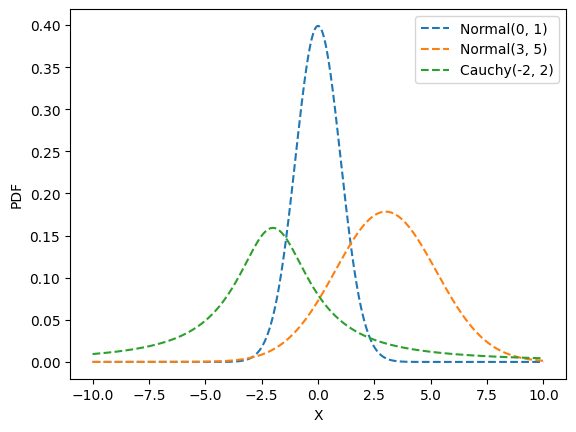
\includegraphics[width=\linewidth]{graph1a}

\subsubsection*{Key Observation}

\subsubsection*{Normal Distribution - \(\mathcal{N}(0, 1)\)}
\begin{itemize}
    \item Has a narrow curve due to low variance, resulting in a high probability
    density around the mean (0).
    \item It has shorter tails - samples drawn from this distribution will be closer
    to the mean.
    \item Does not have long tails - chances of drawing extreme values are low.
\end{itemize}

\subsubsection*{Normal Distribution - \(\mathcal{N}(3, 5)\)}
In comparison with \(\mathcal{N}(0, 1)\),
\begin{itemize}
    \item Has a wider curve due to high variance, resulting in a lower probability
    density around the mean (3).
    \item It has longer tails - a significant number of samples drawn from this
    distribution can be away from the mean (due to high variance).
    \item Tails are slightly longer than \(\mathcal{N}(0, 1)\), but chances of
    drawing extreme values are still low.
\end{itemize}

\subsubsection*{Cauchy Distribution - \(Cauchy(-2, 2)\)}
\begin{itemize}
    \item Has a narrower curve when compared to \(\mathcal{N}(3, 5)\) and has
    longer tails.
    \item This distribution is not symmetric and does not have a mean or variance.
    \item Chances of drawing extreme values are higher when compared to Normal distribution.
\end{itemize}

\newpage
\section*{Question 1.c}
\subsubsection*{QQ plot for samples from \(\mathcal{N}(0, 1)\)}
\includegraphics*[width=\linewidth]{graph1c}
From the QQ plot,
\begin{itemize}
    \item We can observe that the samples drawn from \(\mathcal{N}(0, 1)\)
closely align with the theoretical quantiles of normal distribution.
    \item They form a straight line, indicating that the samples are normally
    distributed.
\end{itemize}

\newpage
\section*{Question 1.d}
\subsubsection*{QQ plot for samples from \(\mathcal{N}(3, 5)\)}
\includegraphics*[width=\linewidth]{graph1d}
From the QQ plot,
\begin{itemize}
    \item We can observe that the samples drawn from \(\mathcal{N}(3, 5)\)
closely align with the theoretical quantiles of normal distribution.
    \item We can see a few points away from the straight line in the plot.
    This is because of the high variance in the distribution.
    \item Ignoring a few outliers, the samples are closer to a straight line,
    indicating that the samples are normally distributed.
\end{itemize}

\newpage
\section*{Question 1.e}
\subsubsection*{QQ plot for samples from \(Cauchy(-2, 2)\)}
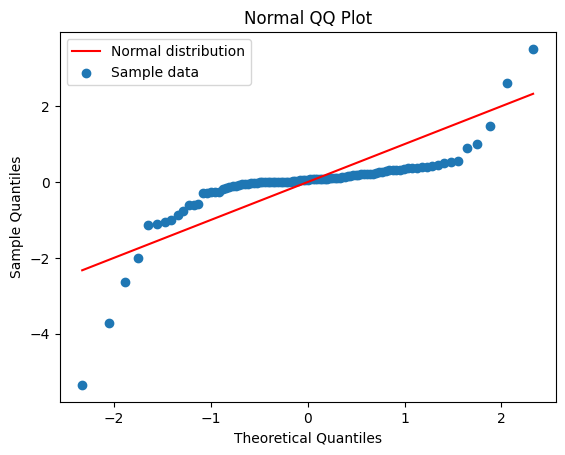
\includegraphics[width=\linewidth]{graph1e}
From the QQ plot,
\begin{itemize}
    \item We can observe that the samples drawn from \(Cauchy(-2, 2)\) do not form
    a straight line - indicating that the samples are not normally distributed.
    \item In addition, we can see multiple outliers in the plot - indicating a
    longer tail.
\end{itemize}

\newpage
\section*{Question 2.a}
Given data: \(x_1 - \bar{x}, x_2 - \bar{x}, x_3 - \bar{x} \dots x_9 - \bar{x}\)
and a mean \(\bar{x}\) of 10 data points.
\\[\baselineskip]
Mean is defined as:

\[\bar{x} = (x_1 + x_2 + x_3 \dots + x_9 + x_{10}) / 10\]
\\
Multiply both sides by 10
\[10 . \bar{x} = (x_1 + x_2 + x_3 \dots + x_9 + x_{10})\]
\\
Subtract \(9.\bar{x}\) from both sides
\[10. \bar{x} - 9.\bar{x} = (x_1 + x_2 + x_3 \dots + x_9 + x_{10}) - 9.\bar{x}\]
\\
Rearrange terms
\[\bar{x} = (x_1 - \bar{x} + x_2 - \bar{x} + x_3 - \bar{x} \dots + x_9 - \bar{x}) + x_{10}\]
\[x_{10} =  (x_1 - \bar{x} + x_2 - \bar{x} + x_3 - \bar{x} \dots + x_9 - \bar{x}) - \bar{x}\]
\\
By substituting the given data points and mean, we get the value of \(x_{10}\).
\\
\section*{Question 2.b}
Sample data points: \(x_1, x_2, x_3 \dots x_9, x_{10}\).
\\
\[s^2 = \frac{\sum_{i=1}^{i=n}(x_i - \bar{x})^2}{n-1}\]
\\
\(\bar{x}\) is the mean of the sample data points and not the population mean.
\\[\baselineskip]
In this case of sample variance, degrees of freedom is n-1 because we use the
sample mean which is a calculated measure from the sample data.
For n = 10, degrees of freedom is 9.
\\[\baselineskip]
Given \(n-1\) data points and a mean of \(n\) data points, we can easily calculate the
missing data point. Which means only \(n-1\) data points can vary, hence we lose
one degree of freedom.

\newpage
\section*{4.a}
\includegraphics*{graph4a}
\\
The plot above shows two datasets sampled from the same distribution
\(Y = 5 + 3.X + \varepsilon\). \(\varepsilon \thicksim \mathcal{N}(0, 1)\)
\\
\begin{itemize}
    \item Both datasets are similar and have a linear relationship.
    \item They have a similar slope and intercept.
    \item There is a small difference between each data point of either dataset
    due to the error term \(\varepsilon\).
    \item The value of error term \(\varepsilon\) is different for each dataset
    as they are drawn independently from the same distribution.
\end{itemize}

\section*{4.b}
Values obtained for dataset 1: \(slope = 2.942\) and \(intercept = 4.856\)
\\
Values obtained for dataset 2: \(slope = 2.951\) and \(intercept = 5.121\)
\\
\begin{itemize}
    \item The outputs are slightly different between the two datasets due to
    the random noise \(\varepsilon\) in generating the data.
    \item The value of error term is different for each dataset as they are
    drawn independently.
    \item This randomness causes the estimated slope to deviate slightly from
    the true value of 3 in each dataset.
\end{itemize}

\newpage
\section*{5.a}
\includegraphics*[width=\linewidth]{graph5a}
\begin{itemize}
    \item From the figure above, we can see that the distribution of sample mean
    is approximately normal regardless of the population distribution.
    \item Between sample sizes of 3 and 5, we can see that the sample distribution
    is approximately normal (somewhat retains the shape of the population distribution).
    \item As the sample size increases, the sample distribution becomes more
    normal and the shape of the population distribution is lost.
    \item This is because the sample mean is an unbiased estimator of the population
    mean and the Central Limit Theorem states that the distribution of sample
    means is approximately normal regardless of the population distribution.
    \item Additionally, we can see that the high variance of the sample distribution
    decreases drastically as the sample size increases.
    \item This is because the more data we sample, the denominator of the sample
    variance increases, but the numerator does not increase by as much (because
    the sample mean remains closer to the population mean).
\end{itemize}

\newpage
\section*{5.e}
\includegraphics*[width=\linewidth]{graph5b}
Plot from data sampled with \(n = 3\) vs \(n = 100\) using normal error term
\(\varepsilon \thicksim \mathcal{N}(0, 1)\).
\begin{itemize}
    \item We can see that the distribution with \(n = 100\) is much narrower
    than the distribution with \(n = 3\).
    \item We see a higher variance in the mean with \(n = 3\) because
    denominator is a smaller number (smaller sample size).
    \item As the sample size increases, the denominator increases and the
    variance decreases (because the numerator does not grow by as much).
\end{itemize}
\includegraphics*[width=\linewidth]{graph5c}
Plot from data sampled with \(n = 3\) vs \(n = 100\) using normal error term
\(\varepsilon \thicksim \mathcal{N}(0, 100)\).
\begin{itemize}
    \item We can see that the distribution with \(n=3\) and
    \(\varepsilon \thicksim \mathcal{N}(0, 100)\) has a wider distribution
    compared to \(\varepsilon \thicksim \mathcal{N}(0, 1)\) for same data size.
    \item This is because of the huge variance in the error term.
    \item But as the sample size increases to 100, we can see that the variance
    has decreased drastically and is similar to the distribution with
    \(\varepsilon \thicksim \mathcal{N}(0, 1)\) for the same sample size.
    \item Even with a high variance in the error term, the mean of 100 numbers
    is closer to the population mean and the variance decreases as the sample
    size increases.
\end{itemize}

\newpage
\includegraphics*[width=\linewidth]{graph5d}
Plot from data sampled with \(n = 3\) vs \(n = 100\) using Chi Squared error term
\(\varepsilon \thicksim \chi^2(10)\).
\begin{itemize}
    \item We can see that the distribution with \(n=100\) is narrower compared
    to the distribution with \(n=3\).
    \item Both of these distributions are approximately normal despite the
    population distribution being Chi Squared.
    \item This is because of the Central Limit Theorem which states that the
    distribution of sample means is approximately normal regardless of the
    population distribution.
\end{itemize}
\subsubsection*{Conclusion}
\begin{itemize}
    \item In summary, the distribution with \(n=3\) and \(\varepsilon \thicksim \mathcal{N}(0, 100)\)
    has the widest distribution due to a high variance in the error term and a small sample size.
    \item As the sample size increases, the variance decreases and the distribution
    is approximately normal.
\end{itemize}

\newpage
\section*{6.a}
\includegraphics*[width=\linewidth]{graph6a}
\begin{itemize}
    \item In the figure above (a), we can see a plot of means from 20 datasets
    sampled from the same distribution, along with their confidence interval.
    \item Each dot on the line represents the mean of one of the 20 datasets and
    the horizontal line around each mean represents the 95\% confidence
    interval for that sample mean.
    \item A confidence interval of 95\% means on an average 95\% of the sample
    means will capture the population mean in their confidence interval.
    \item In the sample above, we can see that only 2 out of 20 intervals fail
    to capture the population mean (as expected).
\end{itemize}

\newpage
\section*{6.b}
\includegraphics*[width=\linewidth]{graph6b}
Plot for data sampled with n = 3 and confidence interval of 95\%.
\begin{itemize}
    \item From the plot above, we can see that not all the confidence intervals
    capture the true slope.
    \item This is expected, as we set the confidence interval to 95\%.
    \item This means that on an average, 5\% of the intervals will not capture
    the true slope.
    \item By setting a higher confidence interval, we can reduce the number of
    intervals that fail to capture the true slope - but this will result in
    wider confidence intervals.
\end{itemize}

\newpage
\section*{6.c}
\includegraphics*[width=\linewidth]{graph6c}
Plot for data sampled with n = 3 and confidence interval of 99\%.
\begin{itemize}
    \item From the plot we can see that the confidence intervals are wider than
    the previous plot. (Ranging from -20 to 20 as opposed to -5 to 10 in the
    previous plot).
    \item This is because we set a higher confidence interval of 99\%. This
    means on an average, only 1\% of the intervals will not capture the true slope.
    \item By setting a higher confidence interval, we reduced the number of intervals
    that do not capture the slope, but the intervals are huge and do not provide
    much information.
\end{itemize}
\end{document}
